\documentclass[a4paper]{llncs}

\usepackage{epsf}     %% om xfig gegenereerde pstexs te includen


% to be removed in final version
\pagestyle{plain}

\title{Formal specification of Gemplus' electronic purse case study}

\author{
  Nestor Cata\~no Collazos
\and
  Marieke Huisman
}

\institute{
  INRIA Sophia-Antipolis, France \\ 
  \email{\{Nestor.Catano, Marieke.Huisman\}@sophia.inria.fr}
}

\newcommand{\noth}{\(\backslash\)\texttt{nothing}}
\newcommand{\fieldsof}{\(\backslash\)\texttt{fields\_of}}
\newcommand{\reach}{\(\backslash\)\texttt{reach}}
\newcommand{\comment}[1]{\marginpar{\framebox{\begin{minipage}{\marginparwidth}{#1}\end{minipage}}}}

\begin{document}
%\input{texdefs.tex}

\maketitle


\begin{abstract}
This paper presents a case study in formal specification of smart card
programs, using ESC/Java. It presents an electronic purse application,
provided by Gemplus, that we have annotated with its functional
specification (\emph{i.e.}~pre-post-conditions, modifies clauses and
class invariants), that are as detailed as possible. The specification
has been based on the informal documentation of the application. The
implementation has been checked \emph{w.r.t.}~the specification, using
ESC/Java.  This revealed several errors or possibilities for
improvement in the code (\emph{e.g.}~removing unnecessary tests). 

The main contribution of this paper is that it shows that relatively
lightweight use of formal specification techniques already can have
serious impact on the quality of a program, and its
documentation. Further, we also present some ideas on how ESC/Java
could be further improved, both
\emph{w.r.t.}~specification and verification.
\end{abstract}

\section{Introduction}
\label{SectIntro}

\paragraph{Background}
When developing a large software application, a significant part of
the work is spent on writing clear and concise documentation. This
documentation serves several purposes: it helps the developers of the
application (to understand the implementation decisions taken by a
colleague, but also to understand ones own decisions after a certain
period of time), and it also is of use when somebody else builds a new
application, using features provided by the application at hand.

However, such program documentation is only useful if it correctly
describes the implementation, thus one would like to have some trust
in its appropriateness. A way to achieve this is to write a formal
specification and then prove the correctness of the implementation
\emph{w.r.t.}~this specification, but this is difficult (as it
requires a good understanding of the semantics underlying the
specification and programming language), and labour-intensive (see
\emph{e.g.}~\cite{HuismanJB00a} for an example of full program
verification). Thus, although it is feasible to do formal
specification and verification, the costs in general do not outweigh
the benefits.

Recently, several suggestions have been made to overcome these
problems. First of all, to encourage application developers to write
formal specifications, specification languages have been developed
which are close to programming languages. The annotation language for
Eiffel~\cite{Meyer97} is the first example of such a specification
language, and recently several annotation languages for Java have been
proposed, following the same strategy:
JML~\cite{LeavensBR99}, Esc/Java~\cite{ESCJavaUrl}, and
the Jass annotation language~\cite{JassUrl}. For JML and Esc/Java,
effort has been put into making these specification languages
converge~\cite{EscJmlDiff}, so that the respective tools can be used
for both languages. Typical for these languages is that
expressions are written as Java expressions, extended with some
specification-specific constructs.

Secondly, together with the Esc/Java language, a static checker has
been developed~\cite{ESCJavaUrl}, which can be used to check simple,
but useful properties. This static checker tries to check that a
program satisfies its annotations, by using a dedicated, automated
theorem prover. This automated theorem prover has been fine-tuned to
find common programming problems like
\texttt{Null\-pointer\-Exception}s, and
\texttt{Array\-Index\-Out\-Of\-Bound\-Exception}s, but it also can be
used to check other annotations. If it cannot establish that a certain
specification is satisfied, it issues a warning. Such a warning does
not necessarily mean that the program is wrong, as the Esc/Java
approach is neither sound, nor complete. When designing the system, a
compromise has been made between soundness, completeness, and
efficiency. The result is an efficient checker, that can increase the
confidence in the correctness of programs, and that finds many common
programming errors. However, if one wishes to establish formally the
correctness of a complicated algorithm, other verification techniques
have to be used, as advocated \emph{e.g.}~in the LOOP
project~\cite{LOOPUrl} or the Jive project~\cite{MeyerP00}. But even
for such complex algorithms it pays to off to use Esc/Java first, in
order to find a first approximation of the errors in the algorithm
and/or specification, before diving into the complete formal
verification.

Annotating programs with Esc/Java specifications can thus be helpful
to create -- reasonably quick -- clear and concise documentation for
a software application, which is according to the implementation.

\paragraph{This paper}
To demonstrate the usefulness of this approach, this paper describes
the Esc/Java annotation of a smart card application case study, which
is the implementation of an electronic purse. The original source code
of this case study comes from Gemplus~\cite{PurseUrl}. In this
paper we discuss the annotations of the source code, and several
possibilities for improvement that we encountered.

The result of this work does not give a fully verified specification,
but it gives a reasonable description of the electronic purse
implementation, which could serve as a basis for further formal
verification, \emph{e.g.}~by using the LOOP compiler.  The main
contribution of this paper is that it shows that by making light
weight use of formal verification techniques, it is feasible to
\emph{(i)} write a formal specification of an application, and
\emph{(ii)} have the implementation checked \emph{w.r.t.}~the 
specification so as to increase confidence in the correctness of the
implementation. When specifying the purse we have
found several (simple) properties which are informally documented, but
are not preserved by the implementation. It is straightforward to
formally specify these properties (typically as class invariants) and
Esc/Java immediately finds the places where these properties are
not preserved in the implementation.

Furthermore, this case study has been one of the first larger case
studies done by using Esc/Java\comment{Is this correct?}, and we found
several points for improvement in the static checker and its
specification language. This lead us to a wish list on improvements in
the specification language and to the development of a checker for
so-called modifiable clauses. This checker will be described in a
separate paper, but we use it in this case study to get further
confidence in the accurateness of the specification.

The remaining of this paper is organised as
follows. Section~\ref{SectGenPurse} describes the general outline of
the case study. Section~\ref{SectStatic} describes the tools that we
used for the static checking of the specification: Esc/Java and our
own modifiability checker. Section~\ref{SectSpecPurse} describes the
annotations of the purse in more detail, and discusses several
interesting aspects of the specification. Section~\ref{SectESC}
comments on the use of ESC/Java and gives suggestions for
improvement. Finally, Section~\ref{SectConcl} gives conclusions and
presents future work.




\section{General outline of the Electronic Purse}
\label{SectGenPurse}
Every \textit{Smart Card} application is split in two
parts$:$ an external application (called terminal) and an
internal one (called applet). The electronic purse is a
\textsc{JavaCard} application which provides to the card holder
the ability to execute bank operations. This application is loaded on
the smart card like an applet. Figure~\ref{fig-cas-pur} shows the
general outline of \textit{the electronic purse}.




\begin{center}
\begin{figure}[hbt]
\rule{\linewidth}{0.3mm}
\\[2.5ex]
\centering
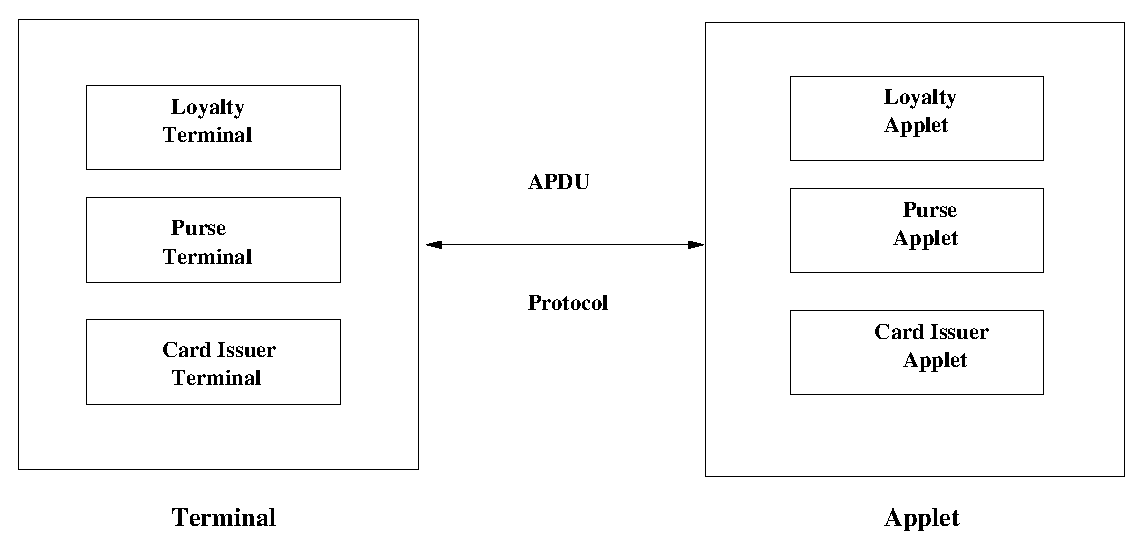
\epsfig{file=figures/javacard.eps, width=11cm, clip=}
\caption{Outline of the purse}
\label{fig-cas-pur}
\rule{\linewidth}{0.3mm}
\end{figure}
\end{center}




The  \texttt{CardIssuer} applet contains personal information of the card
holder and the pin code of the card. The \texttt{Purse}
applet carries out the \textit{credit} and \textit{debit}
operations. This applet also allows the card holder to change the
current currency type defined for the Purse application. The
\textit{currency type} represents the
currency used by the credit and debit operations. Apart from that,
this applet has several mechanisms
which prevent that a command is executed if the applet is not in a
suitable state. The \texttt{Loyalty} applet manages a loyalty counter
that can be increased whenever a purchase is done. When a loyalty
terminal tries to perform a debit on a loyalty, if the balance is not
enough, the loyalty will request other loyalties present in the card
to provide it some points.


\paragraph{\bf The \textit{debit} operation.}
This operation allows to carry out a debit transaction. During a debit 
operation, if severals transactions are carried out in the same
session, it is possible that
the card user presents once his pin code for any transaction lesser than
\texttt{maxDebitWithOutPIN}. The \texttt{maxDebitWithOutPIN} variable
represents the biggest quantity that certain client may credit without
presenting his pin code. For
security reasons, the card holder can do at most
\texttt{maxTransactionWithoutPIN} transactions in a same session. 


\paragraph{\bf The \textit{credit} operation.} This operation allows
to carry out a credit transaction. In spite of fact the purse is
empty, the
card holder can execute a debit operation. In this case, the terminal
sends the bank a request asking for any credit permission. If the card 
holder has some permission, the bank will send to the terminal a
certificate of this.


\paragraph{\bf The \textit{Currency} operation.} The balance is
expressed in a certain currency. When the card holder travels, he has
the possibility to
change the current currency defined for the purse. In this case, the
terminal requests to the bank a
new exchange rate and a certificate. The purse verifies that the bank is 
really the expected bank and validates the exchange rate. After
changing the balance value, the purse must modify all variables related
to the currency.
When a currency change occurs, the purse sends a
\textit{changeCurrency} warning to the loyalties . It is expected than
each loyalty
requests to the purse all logged transactions. After that the purse
may erase
the log transaction file. The purse can be associated to different
loyalties and must differentiate them when the purse is sending
their logged transactions. 






\section{Static checking of Java programs}
\label{SectStatic}


\subsection{\sc \bf Esc/Java}
\label{SubSectEscJava}
\textsc{Esc/Java} is the verification tool developed at
Compaq SRC (Compaq Systems Research Center), which permits to find
 errors in \textsc{Java} programs. \textsc{Esc/Java} detects, at
compile time, common programming errors which usually are not
detected until run time. 

\textsc{Esc/Java} includes an annotation language with which
programmers can express desirable conditions, using light weight
specifications. These desirable conditions represent the conditions
that programmer aspire the program satisfies. For example, one may
give a method precondition which
says that a parameter is not null, or declare an object invariant which
says than an integer field lies between $0$ and the length of some
array field. \textsc{Esc/Java} uses the given annotations in reducing
spurious warnings, and also checks that the program is consistent with 
the given annotations. 

\textsc{Esc/Java} performs \textit{modular checking}, i.e,
\textsc{Esc/Java} checks each class separately. That means that
\textsc{Esc/Java} can be applied to code that calls libraries even if
the code for the libraries is not available. \textsc{Esc/Java} is a
checker for \textsc{Java} programs, which optionally can be annotated
with user supplied pragmas. These pragmas must occur within pragma
containing comments. Furthermore, these pragmas can contain
expressions which are similar to \textsc{Java} expressions. In spite
of this similarity, in \textsc{Esc/Java}, the specification
expressions must be free of subexpressions that, in general, may have
side effects. The following section presents some of the
\textsc{Esc/Java} pragmas, together to some examples of its
utilization. Their full description can be found in~\cite{ESCManual}.

\paragraph{\sc \bf Esc/Java pragmas}
\begin{itemize}
\item{\texttt{==>}.} It is the logical implication. So, \texttt{P
==> Q} is true if and only if \texttt{P} is false or \texttt{Q} is
true, where \texttt{P} and \texttt{Q} are specification expressions of
type \texttt{boolean}. Furthermore, \texttt{<==>} represents the
equivalence relation and \texttt{<=!=>} the in-equivalence one.

\item {($\backslash$\texttt{forall T V; E)} and
($\backslash$\texttt{exists T V; E}).}
They are specification expressions of type \texttt{boolean}. The first one
denotes that \texttt{E} is true for all substitution of values
of type \texttt{T} for the bound variables \texttt{V}. The second one
denotes that \texttt{E} is true for some substitution of values of
type \texttt{T} for the bound variables \texttt{V}.

\item {$\backslash$\texttt{max}.} An expression of the form
\texttt{$\backslash$max(S)}, where \texttt{S} is a specification
expression of type \texttt{Object}, denotes the maximum element of
\texttt{S}. We have a similar definition for the
$\backslash$\texttt{min} pragma.

\item{\texttt{$\backslash$fresh}.} An expression of the form
\texttt{$\backslash$fresh(E)}, where \texttt{E} is a specification
expression of a reference type is a specification expression of type
\texttt{boolean}. Within a postcondition, it denotes that \texttt{E}
is non-null and was not allocated in the pre-state of the routine
call.

\item{\texttt{$\backslash$old($E$)}.} Within a post-condition, it denotes
the value of \texttt{E} in the pre-state of the method invocation. %In
%the following example, the post-condition establishes that the
%variable \texttt{x} will change \texttt{d} units from its original
%value. \textsc{Esc/Java} enables to establish a post-condition by means
%of the \texttt{ensures} clause.\\

%\begin{tabular}{l}
%{\it //@ensures x = $\backslash$old(x) + d} \\
%$\mathtt{public\ void\ {\bf moveX}(int\ d)\{}$ \\
%$\mathtt{\ \ x\ = x\ +\ d\ ;}$ \\
%$\mathtt{\}}$
%\\[3.0ex]
%\end{tabular}

\item {\tt$\backslash$result.} Within a \texttt{ensures} clause
belonging to a non-void method, it represents the value returned by
the method. %In the following example, the clause \texttt{ensures} of
%the method \texttt{getX} establishes that the result of the method will 
%be always the instance variable \texttt{x}. \\


%\begin{tabular}{l}
%{\it //@ensures $\backslash$result == x} \\
%$\mathtt{public\ int\ {\bf getX}(\ )\{}$ \\
%$\mathtt{\ \ return\ x\ ;}$ \\
%$\mathtt{\}}$ 
%\\[3.0ex]
%\end{tabular}

\item{\texttt{$\backslash$nonnullelements}.} An expression of the form
\texttt{$\backslash$nonnullelements(a)}, where \texttt{a} is a
specification expression of array type is a specification expression
of type \texttt{boolean}. It is equivalent to$:$

\texttt{a != null \&\&}
\texttt{($\backslash$forall int i; i >= 0 \&\& i < a.length; a[i] !=
null)}. 
\end{itemize}


%\begin{itemize} 
%\item{\tt ghost} est une instruction de
%d\'eclaration qui permet de d\'eclarer une variables abstraite. Cette
%variable ne peut pas \^etre utilis\'e dans le code \textsc{Java}. \\

%\item{\tt set} est une instruction d'affectation qui permet
%modifier une variable abstraite (\textit{ghost}). Ainsi, la ligne $2$
%dans la classe $Queue$, d\'eclare la variable \texttt{elementType}
%comme \emph{ghost}\footnote{$\backslash${\tt TYPE} repr\'esente un
%type de base.}. \\

%\begin{tabbing}{l}
%ddd\=ddd\=ddd\=ddddddddddddddddddddddd \kill
%\emph{1.}\>$\mathtt{public\ class\ {\bf Queue}\{} $ \\
%\emph{2.}\>\>{\it //@ghost public $\backslash$TYPE elementType ;} \\
%\\
%\emph{3.}\>\>$\mathtt{public\ {\bf Queue}(\ )\ ;} $ \\
%\emph{4.}\>\>$\mathtt{public\ void\ {\bf enqueue}(\ )\ ;} $ \\
%\emph{5.}\>\>$\mathtt{public\ Object\ {\bf dequeque}(\ )\ ;} $ \\
%\emph{6.}\>$\mathtt{\}} $ \\
%\end{tabbing}

%Par cons\'equence, un programmeur peut exprimer son intention de n'utiliser
%la queue \texttt{Queue} qu'avec des \'el\'ements de type \texttt{T}
%par moyen de la d\'eclaration suivante$:$ \\

%\begin{tabbing}{l}
%ddd\=ddd\=ddd\=ddddddddddddddddddddddd \kill
%\>$\mathtt{Queue\ q\ =\ new\ Queue(\ )\ ;}$ \\
%\>{\it //@ set q.elementType $=$ $\backslash$type(T) ;}

%\end{tabbing}
%\end{itemize}

Figure~\ref{fig-add-cur} shows a typical annotation example using the
\textsc{Esc/Java} language. This example was taken from the modeling 
we have done of the \textit{Electronic Purse}. \texttt{addCurrency}
method belongs to \texttt{Currencies} class. This class models all
currency supported by the Purse application. The method
\texttt{addCurrency} adds a new currency to the list of valid
currencies for the Purse. This list is represented by the
\texttt{data} array. The clause
\texttt{modifies} declared in the method's header declares
that the method may modify \texttt{nbData} et
\texttt{data} in the position \texttt{nbData}. More precisely, it
declares that it only may modify these instance variables and the local
variables and formal parameters of the method. The method
\texttt{addCurrency} establishes
two post-conditions by mean of its \texttt{ensure} clauses. The first
one indicates that if \texttt{nbData} have not reached yet the threshold
value $MAX\_DATA$, \texttt{nbData} will increase its value one
unities and the \texttt{data} array in the \texttt{nbData} position
will take the value indicated by the formal parameter
\texttt{cur}. Within these post-conditions, the expressions
\texttt{$\backslash$old(nbData)} refers to \texttt{nbDate} value
before the method invocation.

\begin{figure}[hbt]
\begin{tabbing}
ddd\=ddd\=ddd\=ddd\=ddd\=ddddddddddddddddddddddddddddd \kill
{\it /*@ } \\
\>{\it modifies nbData, data[nbData] ; } \\
\>{\it ensures nbData $==$ ($\backslash$old(nbData) $<$ MAX$\_$DATA $?$ $\backslash$old(nbData)$+$1 $:$$\backslash$old(nbData)) ; } \\
\>{\it ensures data$[\backslash$old(nbData)$]$ $==$ ($\backslash$old(nbData) $<$ MAX$\_$DATA $?$ cur$:$ data$[$nbData$]$) ; } \\
{\it */ } \\
$\mathtt{void\ {\bf addCurrency}(byte\ cur)\ \{}$ \\
\>$\mathtt{if(nbData\ <\ MAX\_DATA) \{}$ \\
\>\>$\mathtt{data[nbData]\ =\ cur\ ;}$ \\
\>\>$\mathtt{nbData++\ ;}$ \\
\>$\mathtt{\}}$ \\
$\mathtt{\}}$ 
\end{tabbing}
\caption{Asserting with {\sc Esc/Java}}
\label{fig-add-cur}
\end{figure}






\subsection{\bf Modifiable Checker}
The functional behavior expressed by mean of \textsc{Esc/Java}
pre-conditions and post-conditions is not enough to reason about
arbitray method calls. Suppose we want to check the method presented by
the figure~\ref{fig-mod-cas}. The specification corresponding to
method \texttt{m} establish that after its invocation the length of
\texttt{myArr} will be $15$. This post-condition is ensured by
the assigment presented on the line $7$. However, the specification of
the
method \texttt{p} must be taken into account for ensuring this
post-condition, due to the instruction on the line $8$. Thus, in a
some manner, the specification of method \texttt{p} must ensure that
its implementation
will not modify the lenght of \texttt{myArray}. That would be possible
with a declaration such as \texttt{modifies $\backslash$nothing}, which
declares that \texttt{p} will not modify any allocation memory. In the 
case of \textsc{Esc/Java}, when a 
situation like this occurs, it assumes effectivaly a
declaration by default \texttt{modifies $\backslash$nothing}, but it
does not check this declarations holds. En consequence, if
method \texttt{p} is overriden in a subclass of \texttt{C} and it
changes the length of \texttt{myArray},
\texttt{Esc/Java} will not complain. Thus, \texttt{Esc/Java} will
accept like true the specification of method \texttt{m} in spite of it
would be wrong. These kind of problems can be overcame if a static checking on
the method overriden is performed. This kind of operation must check
every assignment presented in the method body and establishes wheather
any variable modified for it belongs to set of variables that method
declared or not. More precisely, it must be checked that method body
only modify the variables declared as modifiable, or its formal
parameters o its method variables. 


\begin{figure}[hbt]
\begin{tabbing}
dd\=dddd\=ddd\=ddd \kill
$1$\>{public class {\bf C} \{} \\
$2$\>\>{int [] myArr ;} \\
\\
$3$\>\>{/*@\ normal\_behavior} \\
$4$\>\>\>{ ensures\ myArr.length\ $==$\ 15\ ;} \\
$5$\>\>{ */} \\
$6$\>\>{public void {\bf m}()\{} \\
$7$\>\>\>{myArr = new int [15] ;} \\
$8$\>\>\>{p() ;} \\
$9$\>\>{\}} \\ \\
 
$10$\>\>{/*@ normal$\_$behavior} \\
$11$\>\>\>{ensures true ; }     \\ 
$12$\>\>{ */} \\
$13$\>\>{public void {\bf p}()\{ \} } \\
$14$\>{\}}
\end{tabbing}
\caption{Modifiable clause}
\label{fig-mod-cas}
\end{figure}

Ainsi, for instead, if a declaration such as \texttt{myArray $=$ new
int$[6]$} was occurred inside of the overriden method \texttt{p}, this 
kind of checking would complain due to \texttt{myArray} variable does not
belong to set of variables that method \texttt{m} may
modify\footnote{$\phi$, in this case}.


We have developed a static checker for checking
specification of modifies clauses in \textsc{Java} programs with
assertions \textsc{Esc/Java}. Its implementation follows the static approach
mentioned above and profites the \textsc{Java} Syntaxe for making a
hierarchical checking. This checker will be fully presented in a
separated paper. This checker allows to detect abnomalies situations
such as will be presented in section ??????????. These abnomalies were 
found in the process of checking the modifies clause for the Purse
specifications. 




\section{Specification of the Electronic Purse}
\label{SectSpecPurse}






\subsection{The general specification approach}
ESC/Java forces one to start writing specifications for the classes
that are `used' by many other classes, either because they are used as 
components or because they are inherited from. In the electronic purse 
case study most classes inherit directly from classes as
\emph{e.g.}~\texttt{Object}, \texttt{Exception} or -- in the case of
interfaces -- \texttt{Shareable}, so the inheritance structure is not
very complex. Therefore, we started by specifying classes that
provide basic (and general) features, \emph{e.g.}~those in the
\texttt{utils} package,
that are used by the more classes in the \texttt{purse} package. The
specifications for these basic classes form the basis for the
specification of the more application-specific classes, so it is
important that they are sufficiently detailed.

For every method, we specify the precondition (\texttt{requires} clause
in ESC/Java), the postcondition (\texttt{ensures}), the modifies
clause (\texttt{modifiable}), and the exceptional postcondition
(\texttt{exsures}). ESC/Java does not have a keyword to specify that a
method may not modify any variables, but this is implied by the
absence of a modifies clause. To make our specifications explicit
about this, in such a case we added a comment
\texttt{modifiable \noth;} -- as in JML. Further, ESC/Java requires 
that every exception that is mentioned in the exceptional
postcondition, is also mentioned in the \texttt{throws} clause of the
method. To avoid having to add \texttt{throws} clauses to all methods,
in many cases we chose to have the assertion \texttt{exsures
(Exception) false;} as a comment, without having it checked by
ESC/Java. However, everywhere where there can be any doubt about the
correctness of the \texttt{exsures} clause, we add the \texttt{throws}
clauses and have it checked by ESC/Java.

When writing method specifications, two different approaches can be
taken: either a precondition is given which ensures that no exceptions
will be thrown, or one specifies a light precondition
(\emph{e.g.}~true), and an exceptional postcondition which describes
under which conditions an exception will be thrown. For example, given
the left specification, one has to show that \texttt{P} is satisfied
before the method is called, and then it is guaranteed that the method
cannot produce an exception, while the right hand specification makes
no requirements on the method call, but specifies that if an exception
occurs, this is because \texttt{P} did not hold.
\begin{verbatim}
/*@ modifiable M;                     /*@ modifiable M;
    requires P;                           requires true;
    ensures Q;                            ensures Q;
    exsures (E) false;                    exsures (E) !P;
*/                                    */
void m() {                            void m () {
..                                    ..
}                                     }
\end{verbatim}

In our specifications, we usually follow the first appraoch, which
is close to the \emph{design by contract} approach~\cite{Meyer97},
unless the informal documentation clearly suggests that the second
approach is intended.

Further, we specify appropriate class invariants for each class,
typically restricting the set of legal values for the instance
variables. In some cases, the class invariant immediately follows from
the informal documentation (\emph{e.g.}~the documentation in class
\texttt{Decimal} states
\texttt{the decimal part must be done in the interval [000,999]}), and
in other cases the appropriate class invariant follows from closer
inspection of the code, \emph{e.g.}~a variable is never \texttt{null}.
Section~\ref{SectSpecDetails} discusses the specification of class
invariants in more detail.

Sometimes discrepancies between the informal documentation and the
implementation occur. In general we try to follow the informal
documentation, and we correct the implementation where necessary
(and document these changes). 

In the case study, several functions from the JavaCard
API~\cite{?} are used. When we specify methods using API
functionalities, we use the API specification as constructed by Erik
Poll~\cite{?}. 
In the classes \texttt{Purse} and \texttt{PurseApplet}, several
classes are used that we do not have access to. To overcome this
problem, we ... \comment{What do we do? Does the Houdini paper give a
solution?} 

Our aim is to give a functional specification of the behaviour of the
purse. However, we did not study the algorithms to manage secret keys,
and therefore we only give light weight specification
(\emph{i.e.}~specifying the precondition and modifies clauses, but no
postcondition) of the classes dealing with key generation and
certification. This enables to write and check the specifications of
the classes \texttt{Purse} and \texttt{PurseApplet}. How to specify
and verify cryptographic algorithms is a topic of future research.

We aim at giving specifications which produce a minimal amount of
ESC/Java warnings, but not all warnings can be avoided. Typically, if
a complex control structure occurs in a method (\emph{e.g.}~loops in
which method calls are made) ESC/Java is no longer able to estabish
complicated postconditions. If one wishes to certify these methods,
other verification techniques, as advocated \emph{e.g.}~in the LOOP
project~\cite{LOOPUrl}, should be used. However, in the case study at
hand such complex control structures are not very frequent, and
ESC/Java is able to check most of the specifications without any
problems.

At~\cite{CatanoH01Url} the full annotated version of the purse case
study can be found. In the code it is documented which postconditions
cannot be established by ESC/Java. It is also documented which changes 
we have had to make to the code.



\subsection{Interesting aspects of the specification}\label{SectSpecDetails}
Below, several interesting aspects of the specification are discussed
in more detail. First we will elaborate on some implementation errors
that we found in the purse application.  Then we discuss the
specification of implicit class invariants, and how this can help to
simplify the code. Finally, we discuss some miscellaneous aspects of
the case study, and present some possible improvements. The problems
that we have found probably also would have been found by doing
thorough testing, but using theorem proving techniques one is sure not
to forget some cases. Also, writing the formal specifications forces
one to think very precisely about the intended behaviour of programs,
which helps in finding errors.
\comment{I suggest to merge paragraph coding errors and the one about
the final modifiers into one paragraph. I also move the implicit
invariants and the unnecessary try-catches in one}


\paragraph{Coding errors}
The \texttt{Decimal} class is a purse class and it allows us to
represent a floating point number as
composing by a decimal part and a integer part. These concepts are
represented by the variables \texttt{intPart} and \texttt{decPart}
respectively. This class is shown in the figure~\ref{fig-cla-dec}. The
method \texttt{isGreaterEqualThan} intends to decide when the decimal
represented by \texttt{this} is greater or equal than its parameter
\texttt{d}. Therefore, by mean of a \textsc{Esc/Java} assertion, we
have established a post-condition corresponding to this
specification. This work is done by an \texttt{ensures} comment, which
is shown on the line $8$. 

After running the \textsc{Esc/Java} tool on this method, a warning
signal is activated. This warning suggest that this post-condition
will not be satisfied by the method. The problem is found on the line
$18$. This line must be replaced by \texttt{decPart >=
d.getDecPart()}. In this way, the condition asserted by the clause
\texttt{ensures} will be satisfied.


%\begin{center}
%\begin{figure}[tbh]
%\rule{\linewidth}{0.3mm}
%\rule{0em}{0.1ex}
%\begin{tabbing}
%pub\=lic\=cla\=ssD\=ecimale\=xtendsObject\kill
%\emph{1.}\>$\mathtt{package com.gemplus.pacap.utils\ ;}$ \\
%\\
%\emph{2.}\>$\mathtt{public\ class\ {\bf Decimal}\ extends\ Object\{}$ \\
%\>\>\vdots     \\
%\emph{3.}\>\>{\it /*@ spec$\_$public */} $\mathtt{private\ short\ intPart\ =\
%(short) 0\ ;}$ \\
%\emph{4.}\>\>{\it /*@ spec$\_$public */} $\mathtt{private\ short\ decPart\ =\ (short)\ 0\ ;}$ \\
%\>\>\vdots \\ 
%\emph{5.}\>\>{\it /*@}  \\
%\emph{6.}\>\>\>{\it //modifies $\backslash$nothing} \\
%\emph{7.}\>\>\>{\it requires d $!=$ null;} \\
%\emph{8.}\>\>\>{\it ensures $\backslash$ result $==$ (intPart $>$ d.intPart
%$||$} \\
%\emph{9.}\>\>\>\>{\it (intPart $==$
%d.intPart $\&\&$ (decPart $==$ d.decPart $||$ decPart $>$ d.decPart))) ;} \\ 
%\emph{10.}\>\>{\it */} \\
%\emph{11.}\>\>$\mathtt{public\ boolean\ {\bf isGreaterEqualThan}(Decimal\ d)\{}$ \\
%\emph{12.}\>\>\>$\mathtt{boolean\ resu\ =\ false\ ;}$ \\
%\\
%\emph{13.}\>\>\>$\mathtt{if(intPart\ >\ d.getIntPart())}$ \\
%\emph{14.}\>\>\>\>$\mathtt{resu\ =\ true\ ;}$ \\
%\emph{15.}\>\>\>$\mathtt{else\ if\ (intPart\ <\ d.getIntPart())}$ \\
%\emph{16.}\>\>\>\>$\mathtt{resu\ =\ false\ ;}$ \\
%\emph{17.}\>\>\>$\mathtt{else\ if(intPart\ ==\ d.getIntPart())\{} $        \\
%\emph{18.}\>\>\>\>$\mathtt{if((decPart\ >\ d.getDecPart())\ ||\ (decPart\ >\
%d.getDecPart()))}$ \\
%\emph{19.}\>\>\>\>\>$\mathtt{resu\ =\ true\ ;}$ \\
%\emph{20.}\>\>\>\>$\mathtt{else\ if\ (decPart\ <\ d.getDecPart())}$\\
%\emph{21.}\>\>\>\>\>$\mathtt{resu = false;}$ \\
%\emph{22.}\>\>\>$\mathtt{\}}$ \\
%\emph{23.}\>\>\>$\mathtt{return\ resu\ ;}$ \\
%\emph{24.}\>\>$\mathtt{\}}$ \\
%\>\>\vdots \\
%\emph{25.}\>$\mathtt{\}}$ 
%\end{tabbing}
%\caption{Piece of {\tt Decimal} class}
%\label{fig-cla-dec}
%\rule{\linewidth}{0.3mm}
%\end{figure}
%\end{center}




\paragraph{Final modifiers}
The \texttt{Annee} class allows to represent a \textit{year} in the
\texttt{purse} application. The Figure~\ref{fig-cla-ann} presents its
source code with \textsc{Esc/Java}assertions. This class declares two 
static variables called \texttt{MIN} and \texttt{MAX}, which represent
the minimum and maximum year allowed by the application
respectively. This class declares
also an invariant which relates these values. The static method
\texttt{check} allow us to verify that its parameter is a valid
year. 

The figure~\ref{fig-cla-dat} shows the \texttt{Date} class. This class
represents a date for the application$:$ \texttt{jour}(day),
\texttt{mois}(month), \texttt{annee}(year). We have established some
invariants for this class, which allow the purse application to place
each of them between valide intervals. The method \texttt{setDate}
assigns some values to the internal variables as long as
these variables have valide values, i.e, these variables verify the
conditions expressed by the clauses ensures. In this way, if the
pre-condition is satisfied, the internal variables will be assigned
with the values of their parameters. Otherwise, the method will raise
an \texttt{DateException} exception. This abnormality condition is
declared by the \texttt{exsures} clause. 

\textsc{Esc/Java} complains when it finds a declaration such as$:$ 
\mbox{\tt date.setDate((byte)1, (byte)1, (byte)110);} (where date is a
\texttt{Date} instance). The warning message signals that its third
parameter does not verify the condition established by the clause
\texttt{requires} belonging to the method \texttt{setDate} (line
$5$). This warning is desployed in spite of this call respect the
requires condition, i.e, $110>=99\ \&\&\ 110<= 127$. 

The problem is happend due to the wrong declaration of \textsc{MIN}
and \textsc{MAX} variables belonging to the \texttt{Annee}
class. These variables were not declared as \texttt{final}~\footnote{{\sc
Java} does not allow to change in runtime the value of a final {\tt
final} variable.}. Thus, their values could be changed in runtime by
mean of a direct assignation~\footnote{In fact, due to these variables
are declared are \texttt{public}} and the pre-condition would be not
satisfied. 


The declaration variables as \texttt{static} (commun for all instance)
and \texttt{final} (which can not be changed) prevent us of doing
any assumption that will be not satisfied any more by an
application. This kind of control is carried out by
\textsc{Esc/Java}. 


%\begin{center}
%\begin{figure}[tbh]
%\rule{\linewidth}{0.3mm}
%\\[2.0ex]
%\begin{tabbing}
%pub\=lic\=cla\=ssD\=ate  \kill
%$\mathtt{package\ com.gemplus.pacap.utils\ ;}$ \\
% \\
%$\mathtt{public\ abstract\ class\ {\bf Annee}\ extends\ Object\ \{}$ \\
%\>{\it //@ invariant MIN $<=$ MAX} \\
% \\ 
%\>$\mathtt{public\ static\ byte\ MIN\ =\ (byte)99\ ;} $\\
%\>$\mathtt{public\ static\ byte\ MAX\ =\ (byte)127\ ;} $\\
%\\
%\\
%\>{\it /*@} \\
%\>\>{\it //modifies $\backslash$nothing ;} \\
%\>\>{\it requires true ;} \\
%\>\>{\it ensures $\backslash$result $==$ (j $>=$ MIN $\&\&$ j $<=$ MAX) ;} \\
%\>\>{\it //exsures (RuntimeException)false ;} \\
%\>*/ \\
%\>$\mathtt{public\ static\ boolean\ {\bf check}(byte\ j)\ \{} $ \\
%\>\>$\mathtt{return\ ((j\ >=\ Annee.MIN)\ \&\&\ (j\ <=\ Annee.MAX))\ ;}$  \\
%\>$\mathtt{\}} $ \\
%$\mathtt{\}} $ \\
%\end{tabbing}
%\caption{{\tt Annee} class}
%\label{fig-cla-ann}
%\rule{\linewidth}{0.3mm}
%\end{figure}
%\end{center}





%\begin{center}
%\begin{figure}[tbh]
%\rule{\linewidth}{0.3mm}
%\\[2.0ex]
%\begin{tabbing}
%pub\=lic\=cla\=ssD\=ate\=ext\=endsObject  \kill
%$\mathtt{public\ class\ {\bf Date}\ extends\ Object\ \{}$ \\

%\>{\it /*@} \\
%\>\>{\it invariant jour $>=$ Jour.MIN $\&\&$ jour $<=$ Jour.MAX ;} \\	
%\>\>{\it invariant mois $>=$ Mois.MIN $\&\&$ mois $<=$ Mois.MAX ;} \\
%\>\>{\it invariant annee $>=$ Annee.MIN $\&\&$ annee $<=$ Annee.MAX ;} \\
%\>{\it */}
%\\
%\\
%\>{\it /*@ spec$\_$public */} $\mathtt{private\ byte\ jour\ =\ Jour.MIN\ ;}$ \\
%\>{\it /*@ spec$\_$public */} $\mathtt{private\ byte\ mois\ =\ Mois.MIN\ ; }$ \\   
%\>{\it /*@ spec$\_$public */} $\mathtt{private\ byte\ annee\ =\ Annee.MIN\ ;}$ \\
%\\ 
%\\
%\emph{1. }\>{\it /*@} \\ 
%\emph{2. }\>\>{\it modifies jour, mois, annee ;} \\
%\emph{3. }\>\>{\it requires j $>=$ Jour.MIN  $\&\&$ j $<=$ Jour.MAX ;} \\
%\emph{4. }\>\>{\it requires m $>=$ Mois.MIN  $\&\&$ m $<=$ Mois.MAX ;} \\
%\emph{5. }\>\>{\it requires a $>=$ Annee.MIN $\&\&$ a $<=$ Annee.MAX ;} \\
%\emph{6. }\>\>{\it ensures jour $==$ j $\&\&$ annee $==$ a $\&\&$ mois $==$ m ;} \\
%\emph{7. }\>\>{\it exsures (DateException) false ;} \\
%\emph{8. }\>{\it */} \\
%\>$\mathtt{public\ void\ {\bf setDate}(byte\ j,\ byte\ m,\ byte\ a)\ throws\ DateException\{}$ \\
%\>\>{\it // check the day } \\        
%\>\>$\mathtt{if(!Jour.check(j)) \{}$ \\
%\>\>\>$\mathtt{DateException.throwIt(DateException.ERREUR\_JOUR)\ ;}$ \\
%\>\>$\mathtt{\}else\ \{}$ \\
%\>\>\>{\it // check the month} \\
%\>\>\>$\mathtt{if(!Mois.check(m))\ \{}$\\
%\>\>\>\>$\mathtt{DateException.throwIt(DateException.ERREUR\_MOIS)\ ;}$ \\
%\>\>\>$\mathtt{\}else\ \{}$ \\
%\>\>\>\>{\it // check the year} \\
%\>\>\>\>$\mathtt{if(!Annee.check(a)) \{}$ \\
%\>\>\>\>\>$\mathtt{DateException.throwIt(DateException.ERREUR\_ANNEE)\ ;}$ \\
%\>\>\>\>$\mathtt{\}else\ \{}$ \\
%\>\>\>\>\>{\it $\slash \slash$ all is good} \\
%\>\>\>\>\>$\mathtt{jour\ =\ j\ ;} $\\
%\>\>\>\>\>$\mathtt{mois\ =\ m\ ;} $\\
%\>\>\>\>\>$\mathtt{annee\ =\ a\ ;} $\\
%\>\>\>\>$\mathtt{\}}$ \\
%\>\>\>$\mathtt{\}} $\\
%\>\>$\mathtt{\}} $\\
%\>$\mathtt{\}} $\\
%\>$\vdots$ \\
%$\mathtt{\}}$ \\
%\end{tabbing}
%\caption{{\tt Date} class}
%\label{fig-cla-dat}
%\rule{\linewidth}{0.3mm}
%\end{figure}
%\end{center}






\paragraph{Class invariants}
Typically, invariants are used to restrict the state space of a class,
\emph{i.e.}~the set of allowed values for its instance variables. The
most common example is an invariant which states that a reference
variable may never be a null pointer, \emph{e.g.}~the variable
\texttt{Purse purse}, as declared in the class \texttt{PurseApplet}
should never be null.
\begin{verbatim}
//@ invariant purse != null;
\end{verbatim}
Another common example of an invariant is to restrict the possible
values of a numeric variable to a certain range. As remarked above, in
the class \texttt{Decimal} it says that the value of the decimal
fraction must be between 0 and 999. Inspection of the code teaches us
that the integer part of the decimal number is supposed to be a
positive short, and combining this gives the following class
invariant\footnote{\texttt{MAX\_DECIMAL\_NUMBER} is equivalent to the
maximal value of a short and the clause \texttt{intPart <=
MAX\_DECIMAL\_NUMBER} of the invariant will thus be
ensured by the type of the variable. We chose to state this explicitly
for clearity of specification.}
\begin{verbatim}
/*@
  invariant decPart >= 0 && decPart < PRECISION ;
  invariant intPart >= 0 && intPart <= MAX_DECIMAL_NUMBER;
*/
\end{verbatim}

In Java(Card) there are no enumeration types, and to simulate them
typically several constants are defined with suggestive names, and a
variable is silently assumed to contain always one of these
values. This implicit assumption can be made explicit by specifying
invariants. For example, the class \texttt{Transaction} contains the
following declarations.
\begin{verbatim}
/* the transaction status*/
public static final byte INDETERMINE		= (byte)0;

/* the transaction status*/
public static final byte TYPE_CREDIT		= (byte)50;
/* the transaction status*/
public static final byte TYPE_DEBIT		= (byte)51;
    
/* the transaction type: debit or credit*/
/*@ spec_public*/ private byte type;
\end{verbatim}

This suggests that the variable \texttt{type} always should have a
value \texttt{TYPE\_CREDIT} or \texttt{TYPE\_DEBIT}. However, in the
code (in the method \texttt{reset()}), an assignment \texttt{type =
INDETERMINE;} occurs, suggesting that this is also a correct value for 
\texttt{type}. Having a specification which states the allowed values
for this variable avoids all confusion\footnote{However, notice that it 
does not prevent that other -- arbitrary -- variables can have one of
these values, thus this does not completely simulate enumeration
types.}.
\begin{verbatim}
/*@ invariant type == INDETERMINE ||
              type == TYPE_CREDIT || 
              type == TYPE_DEBIT;
*/
\end{verbatim}

Invariants of this kind occur often in the specification of the
electronic purse. It is easy to specify them, and useful as well, as
there are examples in the electronic purse where such implicit
invariants are violated.
For example, the class \texttt{AccessCondition} declares constants to
state the different access conditions for the actions in the
purse. Following~\cite{?}, variables that denote access conditions
should be restricted as follows.
\begin{verbatim}
/*@ invariant condition == FREE ||
              condition == LOCKED ||
              condition == SECRET_CODE ||
              condition == SECURE_MESSAGING ||
              condition == (SECRET_CODE | SECURE_MESSAGING);
*/
\end{verbatim}

However, in the constructor of this class, the variable
\texttt{condition} is set to 0, which breaks this
invariant. Correcting this and maintaining the invariant also allows
to improve other parts of the implementation in this class. For
example, in the method \texttt{verify()}, the following statement
occurs:
\begin{verbatim}
switch(condition) {
  case FREE: ...
  case SECRET_CODE: ...
  case SECURE_MESSAGING: ...
  case SECRET_CODE | SECURE_MESSAGING: ...
  case LOCKED: ...
  default: //@ assert false;
           t = AccessConditionException.CONDITION_COURANTE_INVALIDE;
           AccessConditionException.throwIt(t);
  }
\end{verbatim}
Because of the invariant we know that the default case will never
be reached (as assured by the \texttt{//@ assert false;} annotation,
which states that false should hold, every time this program point is
reached), and thus that the exception never will be thrown. Thus, the
default case can be removed from the code.

Similar cases occur frequently with \texttt{try-catch} statements. An
operation is executed within a \texttt{try}, but as the class invariants
assure that the operation never will throw an exception, the
\texttt{catch} clause will never be executed. In the specification, we 
have annotated these cases with \texttt{//@ assert false;}. We think
that the removal of this ``dead code'' can improve the readability of
the class, and -- which is important for smart cards -- can reduce the 
size of the byte code.


\paragraph{Miscellaneous aspects of the specification}
There are many other aspects of the specification that are worth
mentioning. Here we mention some.

\begin{itemize}
\item As explained above, in the class \texttt{Decimal}, two shorts
are maintained denoting the integer and the decimal part
(\texttt{intPart} and \texttt{decPart}, respectively) of a decimal
number. The integer part ranges between 0 and
\texttt{MAX\_DECIMAL\_NUMBER} (which is 32767, the maximal value for
shorts). It is left unspecified whether numbers such as
\texttt{MAX\_DECIMAL\_NUMBER}.999 are allowed. However, 
a method \texttt{round()} is defined, which
according to the documentation returns a decimal number with
\texttt{decPart} set to 0 and \texttt{intPart} set to the closest
integer value. An obvious specification of this method reads as
follows:
\begin{verbatim}
/*@ 
  modifies intPart, decPart;
  ensures decPart == 0;
  ensures intPart == (\old(decPart) >= (PRECISION/2) ?
                          (short)(\old(intPart) + 1) :
                             (short)(\old(intPart)))
*/
public Decimal round(){ ... }
\end{verbatim}
But, as pointed out by ESC/Java, an implementation of this
specification breaks the class invariant \texttt{intPart >= 0}. The
counterexample that is produced has
\texttt{intPart} set to \texttt{MAX\_DECIMAL\_NUMBER} and
\texttt{decPart} \emph{e.g.}~to 999. Possible solutions are to
specify explicitly the outcome of \texttt{round()} in the case that
\texttt{intPart == MAX\_DECIMAL\_NUMBER}, or to restrict the set of
valid decimal numbers, by further strengthening of the class invariant
through addition of the following clause:
\begin{verbatim}
//@ invariant intPart == MAX_DECIMAL_NUMBER ==> decPart == 0;
\end{verbatim}
We chose this last solution. 

\item Among the developers of the electronic purse application there
apparently have been different ideas about the implementation of the
class \texttt{Decimal}. The implementation of several
\texttt{setValue(...)} methods
reveal that \texttt{intPart} is assumed to be greater or equal than
0, but on the other hand there are methods
\texttt{isNegatif()} and \texttt{isPositif()}, which test whether a
decimal value is negative or positive, respectively. As we specify
that \texttt{intPart} should be greater or equal than
0\footnote{\emph{cf.} our email exchange with H. Martin, Gemplus.}
these methods become obsolete. We can show this by specifying
that their results can be predicted, \emph{e.g.}~\texttt{isNegatif()} we 
specify as follows:
\begin{verbatim}
/*@ 
  ensures \result == false;
*/
public boolean isNegatif(){ ... }
\end{verbatim}


\item Two classes, \texttt{TransactionRecord} and
\texttt{ExchangeRecord} implement a cyclic table (of
\texttt{Transaction}s and
\texttt{ExchangeSession}s (representing currency changes),
respectively).  These implementations are clearly copied from each
other, but this is nowhere documented. Also the fact that a
cyclic datastructure is implemented is not very well documented. Class
\texttt{TransactionRecord} contains a single remark that it is
implemented as a cyclic table, and for class
\texttt{ExchangeRecord} this is only stated in the documentation of a
private method. Also, no specification of the operations on the cyclic
datastructure are given.

As a result, in class \texttt{ExchangeRecord}, part of the code that
is crucial for the cyclidity has been commented out by other
developers of the electronic purse. Having a formal specification
would probably have been helpful to explain the complexity of the
implementation to the other developers, and the 'wrong correction'
would have been signalled earlier\footnote{Of course, having a general 
implementation of a cyclic table and instantiating this for the
different kinds of data would have been even more elegant.}.

Finally, when writing the formal specifications of the cyclic tables,
we found an error in the implementation. When a delete operation is
called for an element that is not in the range of the table, the
operation nevertheless will be executed and as a side-effect it will
corrupt the table by erroneously moving its first element outside the
range of the table.
\end{itemize}


\section{On the use of ESC/Java}
\label{SectESC}
We find ESC/Java a useful tool, that is pleasant to work
with, but nevertheless we have some suggestions for improvements. In
particular, we feel that certain specification constructs that are
available in JML~\cite{LeavensBR99}, should be provided in ESC/Java as 
well. They could be implemented as syntactic sugar only, but would be
very useful to give clear and concise specifications.
First of all, we would like to be able to use method names in
specifications, as is allowed in JML for so-called
\emph{pure} methods, \emph{i.e.}~methods without
side-effects. Further, we would like to have some extra specification
constructs for modifies clauses, \emph{e.g.}~\fieldsof, to denote all
the fields of an object, and \noth. Also we feel that having some
extra quantifiers, such as \texttt{\(\backslash\)min},
\texttt{\(\backslash\)max}, and \texttt{\(\backslash\)choose} would be 
very useful.

\begin{figure}[tbh]
\begin{verbatim}
    /*@
      modifies \fields_of(this), \fields_of(date), \fields_of(heure),
               id[*], terminalTC[*], terminalSN[*];
      requires es != null ;
      requires es.id != terminalTC & es.id != terminalSN &
               es.terminalTC != terminalSN;
      ensures this.equal(es);
      exsures (TransactionException e) 
                  e._reason == TransactionException.BUFFER_FULL 
                  && JCSystem._transactionDepth == 1; 
      exsures (NullPointerException) false;
      exsures (ArrayIndexOutOfBoundsException) false;
    */
    void clone(ExchangeSession es) { ...
    } 
\end{verbatim}
\caption{Specification of \texttt{clone} in \texttt{ExchangeSession}
in ideal ESC/Java}
\label{FigIdealESC}
\end{figure}

Figure~\ref{FigIdealESC} shows as an example how we would like the
specification of the method \texttt{clone()} in class
\texttt{ExchangeSession} to be (see~\cite{CatanoH01Url} for the
ESC/Java specification as it is). We only specify that the fields of
the current class all may be modified, without explicitly mentioning
them. As the fields of the component classes \texttt{date} and
\texttt{heure} may be modified as well, we mention this
explicitly. Similarly, we mention explicitly that the elements in the
arrays \texttt{id}, \texttt{terminalTC} and \texttt{terminalSN} may be
modified\footnote{In JML one can write this modifies clause also
simply as \fieldsof(\reach), which would probably be useful in many
cases as well, but has a more complex semantics.}. Further, instead of
having postconditions stating that all the fields are ensured to be
equal to the corresponding fields of \texttt{es}, this is denoted by
writing \texttt{this.equal(es)}, where \texttt{equal} is overwritten
appropriately in \texttt{ExchangeSession}.

Further, we feel that it would be an improvement if ESC/Java would
deal more precisely with arithmetic operations (also on bytes and
shorts). For example, several times we needed that for \emph{e.g.}~a
byte \texttt{b} with a value between 0 and 10, after the operation
\texttt{b++} this variable still has a positive value. 

Finally, it would be nice if one could specify runtime exceptions in
\texttt{exsures} clauses, while they are not mentioned in the
\texttt{throws} clause of the method.

\section{Conclusions}
\label{SectConcl}

We have presented a case study in formal specification of smart card
programs, using ESC/Java. We have taken an electronic purse
application and annotated it with a functional specification,
describing its behaviour, basing ourselves on the informal
documentation of the application. We have checked the implementation
\emph{w.r.t.}~the specification, using ESC/Java, thereby revealing
several errors in the implementation. Using ESC/Java we were also able 
to find that some parts of the program will never be reached, thus
allowing reduction of the code size -- which is important for smart
card applications. 

The errors that we found in general are not very complex, they could
have been found by careful code-inspection or testing. But, writing
the formal specification forces one to do code-inspection, and having
the theorem prover ensures that all possible cases will be
considered, when checking the specification.

The specifications that we have constructed for the electronic purse
application are not very complex, but describe the functional
behaviour of methods as precisely as possible. Nevertheless, we found
errors in the code, and we would like to emphasise that even simple
formal verification can help significantly to increase confidence in a
program. In particular, explicitly specifying class invariants turns
out to be very useful.

\paragraph{Future work} We plan to work in the field of
specification languages for Java: how to improve them, and how to
develop appropriate verification techniques for them. In particular,
we will focus on the following points.
\begin{itemize}
\item We plan to develop a full smart card application from scratch, with
annotations. We are interested whether this will affect the quality of 
the specification and/or the program. Also we would like to know how
easy it is to construct the specifications at the same time as
developing the code. Is it useful, because one can get immediate
feedback on an implementation, or is it a burden because more time
is spend on keeping the the specification up-to-date, then on
implementing the program.
\item Future versions of JavaCard will probably allow
multi-threading. Therefore we plan to study how to ESC/Java (and JML)
can be used to specify (and check) concurrent programs.
\item Related with this is that we will work on an extension of JML with
temporal logic. Currently we are studying how to integrate temporal
logic in the specification language, future work will be to study
appropriate verification techniques.
\item Most loop structures that are used in typical smart card
programs are very restricted and it is relatively easy to show their
termination. We plan to develop an automated verification technique for
termination of loops in the tradition of ESC/Java, covering the most
common cases.
\item We skipped the cryptographic aspects of the application at
hand. It is future work to see whether ESC/Java (or JML) is useful to
specify such algorithms more precisely -- and to develop appropriate
(automated) verification techniques.
\end{itemize}

\bibliographystyle{plain}
\bibliography{../specification}

\end{document}

